\scanpage{43}
\begin{center}- 17 -\end{center}
\hfill n$^\circ$ 276
\[
w:\widehat{E/F}\longrightarrow\widehat{\hat E/\hat F}
\]
Il est clair que $w\circ v$ n'est autre que l'application canonique de $\hat E/\hat F$ dans son complété ; si de plus l'on prolonge $v$ en une représentation
\[
\hat v:\widehat{\hat E/\hat F}\longrightarrow\widehat{E/F}
\]
alors $\hat v\circ w$ est l'identité, puisque c'est déjà l'identité sur $E/F$.

\uline{Si} $\hat E/\hat F$ \uline{est complet}, il résulte de ce qui précède que $v$ et $w$ sont des représentations inverses l'une de l'autre, autrement dit que $v$ est un isomorphisme du groupe topologique $\hat E/\hat F$ sur le groupe topologique $\widehat{E/F}$. D'après la prop.4, de \uline{Top. Gén.} Chap.IX, \S3, ce sera toujours le cas si le groupe $E$ est \uline{métrisable} puisqu'alors $\hat F$ est un sous-groupe fermé du groupe métrisable et complet $\hat E$. Il en sera de même plus généralement si la topologie de $E$ peut être définie à l'aide d'un écart.

On déduit de là le résultat suivant :

\uline{Lemme} 1 - \uline{Soient} $E,F,G$ \uline{trois groupes topologiques abéliens métrisables}, $u:E\longrightarrow F$ \uline{et} $v:F\longrightarrow G$ \uline{deux homomorphismes topologiques telle que la suite de groupes abéliens} $E\xrightarrow{u}F\xrightarrow{v}G$ \uline{soit} \uuline{exacte}. \uline{Alors} $\hat u:\hat E\to\hat F$ \uline{et} $\hat v:\hat F\longrightarrow\hat G$ \uline{sont des homomorphismes topologiques et la suite} $\hat E\xrightarrow{\hat u}\hat F\xrightarrow{\hat v}\hat G$ \uline{est exacte}.
\margin{\figure{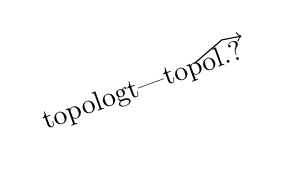
\begin{tikzpicture}\node[rotate=20] at (0,0) {\unsure{topologt|topol.?}};\draw[->] (.65,.3)--(1,.6)--(1.25,.65);\end{tikzpicture}}}

On a vu en effet, que le lemme 1 est vrai lorsque $u$ est injectif et $v$ surjectif. Or dans le cas général, la suite exacte donnée se décompose en suites exactes partielles,
\diagram{\begin{tikzcd}[column sep=small]N\arrow[r]&E\arrow[r]&I\end{tikzcd}\ ;\quad\begin{tikzcd}[column sep=small]I\arrow[r]&F\arrow[r]&J\end{tikzcd}\ ;\quad\begin{tikzcd}[column sep=small]J\arrow[r]&G\arrow[r]&K\end{tikzcd}}
qui rentrent dans ce cas particulier, et auxquelles le lemme 1 est donc applicable ; d'où évidemment le résultat cherché puisque le composé de deux homomorphismes est un homomorphisme.

Ces préliminaires sur les groupes topologiques étant rappelés, considérons
\mspage{42}
